\section{Entidades e Processos}

O trabalho tem por propósito explorar a emergência de distribuições de
preferências fundamentando-se no diálogo entre a Teoria Política Espacial e a
área de Dinâmicas de Opinião. Não temos por propósito um modelo que seja
preditivo, mas que capture microfundamentos relevantes, como viés de confirmação
e confiança nas crenças, e gere distribuições de preferência plausíveis, no
sentido delimitado no Capítulo 1. O trabalho propõe, portanto, um modelo que
abra a caixa-preta do processo de socialização que leva a cristalização de
direcionamentos, ou posicionamentos, ideológicos.

A Teoria Geométrica de política modela as preferências dos agentes como relações
em um espaço contínuo, as quais, em ambientes macro, são construídas por meio da
agregação das atitudes, crenças, posicionamentos, ou simplesmente opiniões dos
agentes em diferentes questões (\textit{issues}). As preferências dos agentes
numa dimensão são, assim, o sumário de um \textit{perfil ideológico} do agente
sobre questões.

Para gerar a distribuição de pontos ideais, contudo, não precisamos especificar
qual a função de utilidade centrada nele, já que não é interesse do trabalho
modelar a tomada de decisão que o pressuporia, por exemplo a escolha de um
candidato. Como discutido no Capítulo 1, é possível atribuir diferentes funções
de utilidade aos agentes, mas o pressuposto modal é que a função vai ter um
máximo e será simétrica \cite{eguia2013spatial, carroll2013structure}. Como não
é um modelo de tomada de decisão, mas sim um modelo de surgimento de
posicionamentos ideológicos, não é necessário adicionar mais um elemento,
funções de utilidade, que simplesmente alargaria o espaço de parâmetros e não
seria utilizado na simulação. Contudo, modelos futuros que busquem ligar, por
exemplo, a distribuição de preferências com a escolha de candidatos/partidos
poderiam fazer essa atribuição.

%Assumimos, portanto, que as preferências dos
%agentes na dimensão são de pico-único, o pressuposto modal, desde
%\citeonline{black1958theory}, na literatura em modelos fortemente espaciais, e
%em trabalhos empíricos em estimação de pontos ideais \cite{carroll2013structure,
% armstrong2014analyzing, schofield1998nash}.

Pensar os agentes como tendo ideais derivados de posicionamentos em outras
questões tem por base dois fundamentos. O primeiro é que esse elemento a mais, em
comparativo aos modelos de \citeonline{deffuant2000mixing} e de
\citeonline{martins2012bayesian}, nos permite ser mais condizentes com a
literatura discutida no Capítulo 1 em contraposição à equiparação do ponto ideal
a uma opinião. Isto é, os pontos ideais dos agentes vão mudar ao longo da
simulação, mas isso ocorre devido à mudança nas suas crenças. É uma
mudança assim indireta e condizente com a noção de que a ideologia do agente é
um atributo extrínseco. O segundo fundamento é que essa modificação tem por
implicação a capacidade de adicionar outros elementos à dinâmica do modelo.

Sendo assim, cada agente na nossa população vai ter por atributo um perfil
ideológico\footnote{Nisso o modelo aproxima-se do modelo de
  \citeonline{axelrod1997dissemination}, no qual os agentes tem por atributo um
  conjunto de traços.} \(I\), onde \(I_i = (f_i(\theta_1), \ldots, f_i(\theta_n)) \). Os
elementos de \(I\) são as crenças dos agentes em cada questão. Seguindo
\citeonline{martins2012bayesian}, vamos pressupor que os agentes têm uma
probabilidade subjetiva sobre cada questão \(\theta\), e uma opinião \( o_i =
E_i[\theta]\) e incerteza \( \sigma_i^2 = E[\sigma^2] - E_ i[\theta]^2\) associados. O ponto ideal
\(x\) do agente vai ser a média aritmética das opiniões dele em \(I\). Do ponto
de vista da implementação o atributo \(I\) é reduzido a um conjunto de pares
\(I_i = ((o_{i,1},\sigma_{i,1}^2), \ldots, (o_{i,n}, \sigma_{i,n}^2) )\), sendo \(\sigma^2\) global.
Se \(o\) for retirado de uma distribuição uniforme (U[0,1]), como em
\citeonline{deffuant2000mixing}, quanto mais vezes fazemos esse sorteio (quanto
maior o número de questões), pela Lei dos Grandes Números, mais centrada a média
aritmética ( \(x_i = \frac{1}{n}\sum_{k=1}^{n} o_k\)) vai ser do valor esperado da
distribuição (0.5). Isso significa que já na condição inicial os agentes seriam
de centro. Para que isso não ocorra associamos para cada agente uma distribuição
Beta, com \(\alpha\)s e \(\beta\)s entre 1.1 e 100. Destas distribuições sorteamos os
valores de \(o_i\) para cada questão, de forma que as opiniões são
correlacionadas e as distribuições são centradas em diferentes pontos do espaço,
como ilustrado na Figura \ref{fig:betas100}:

\begin{figure}[H]
  \centering
  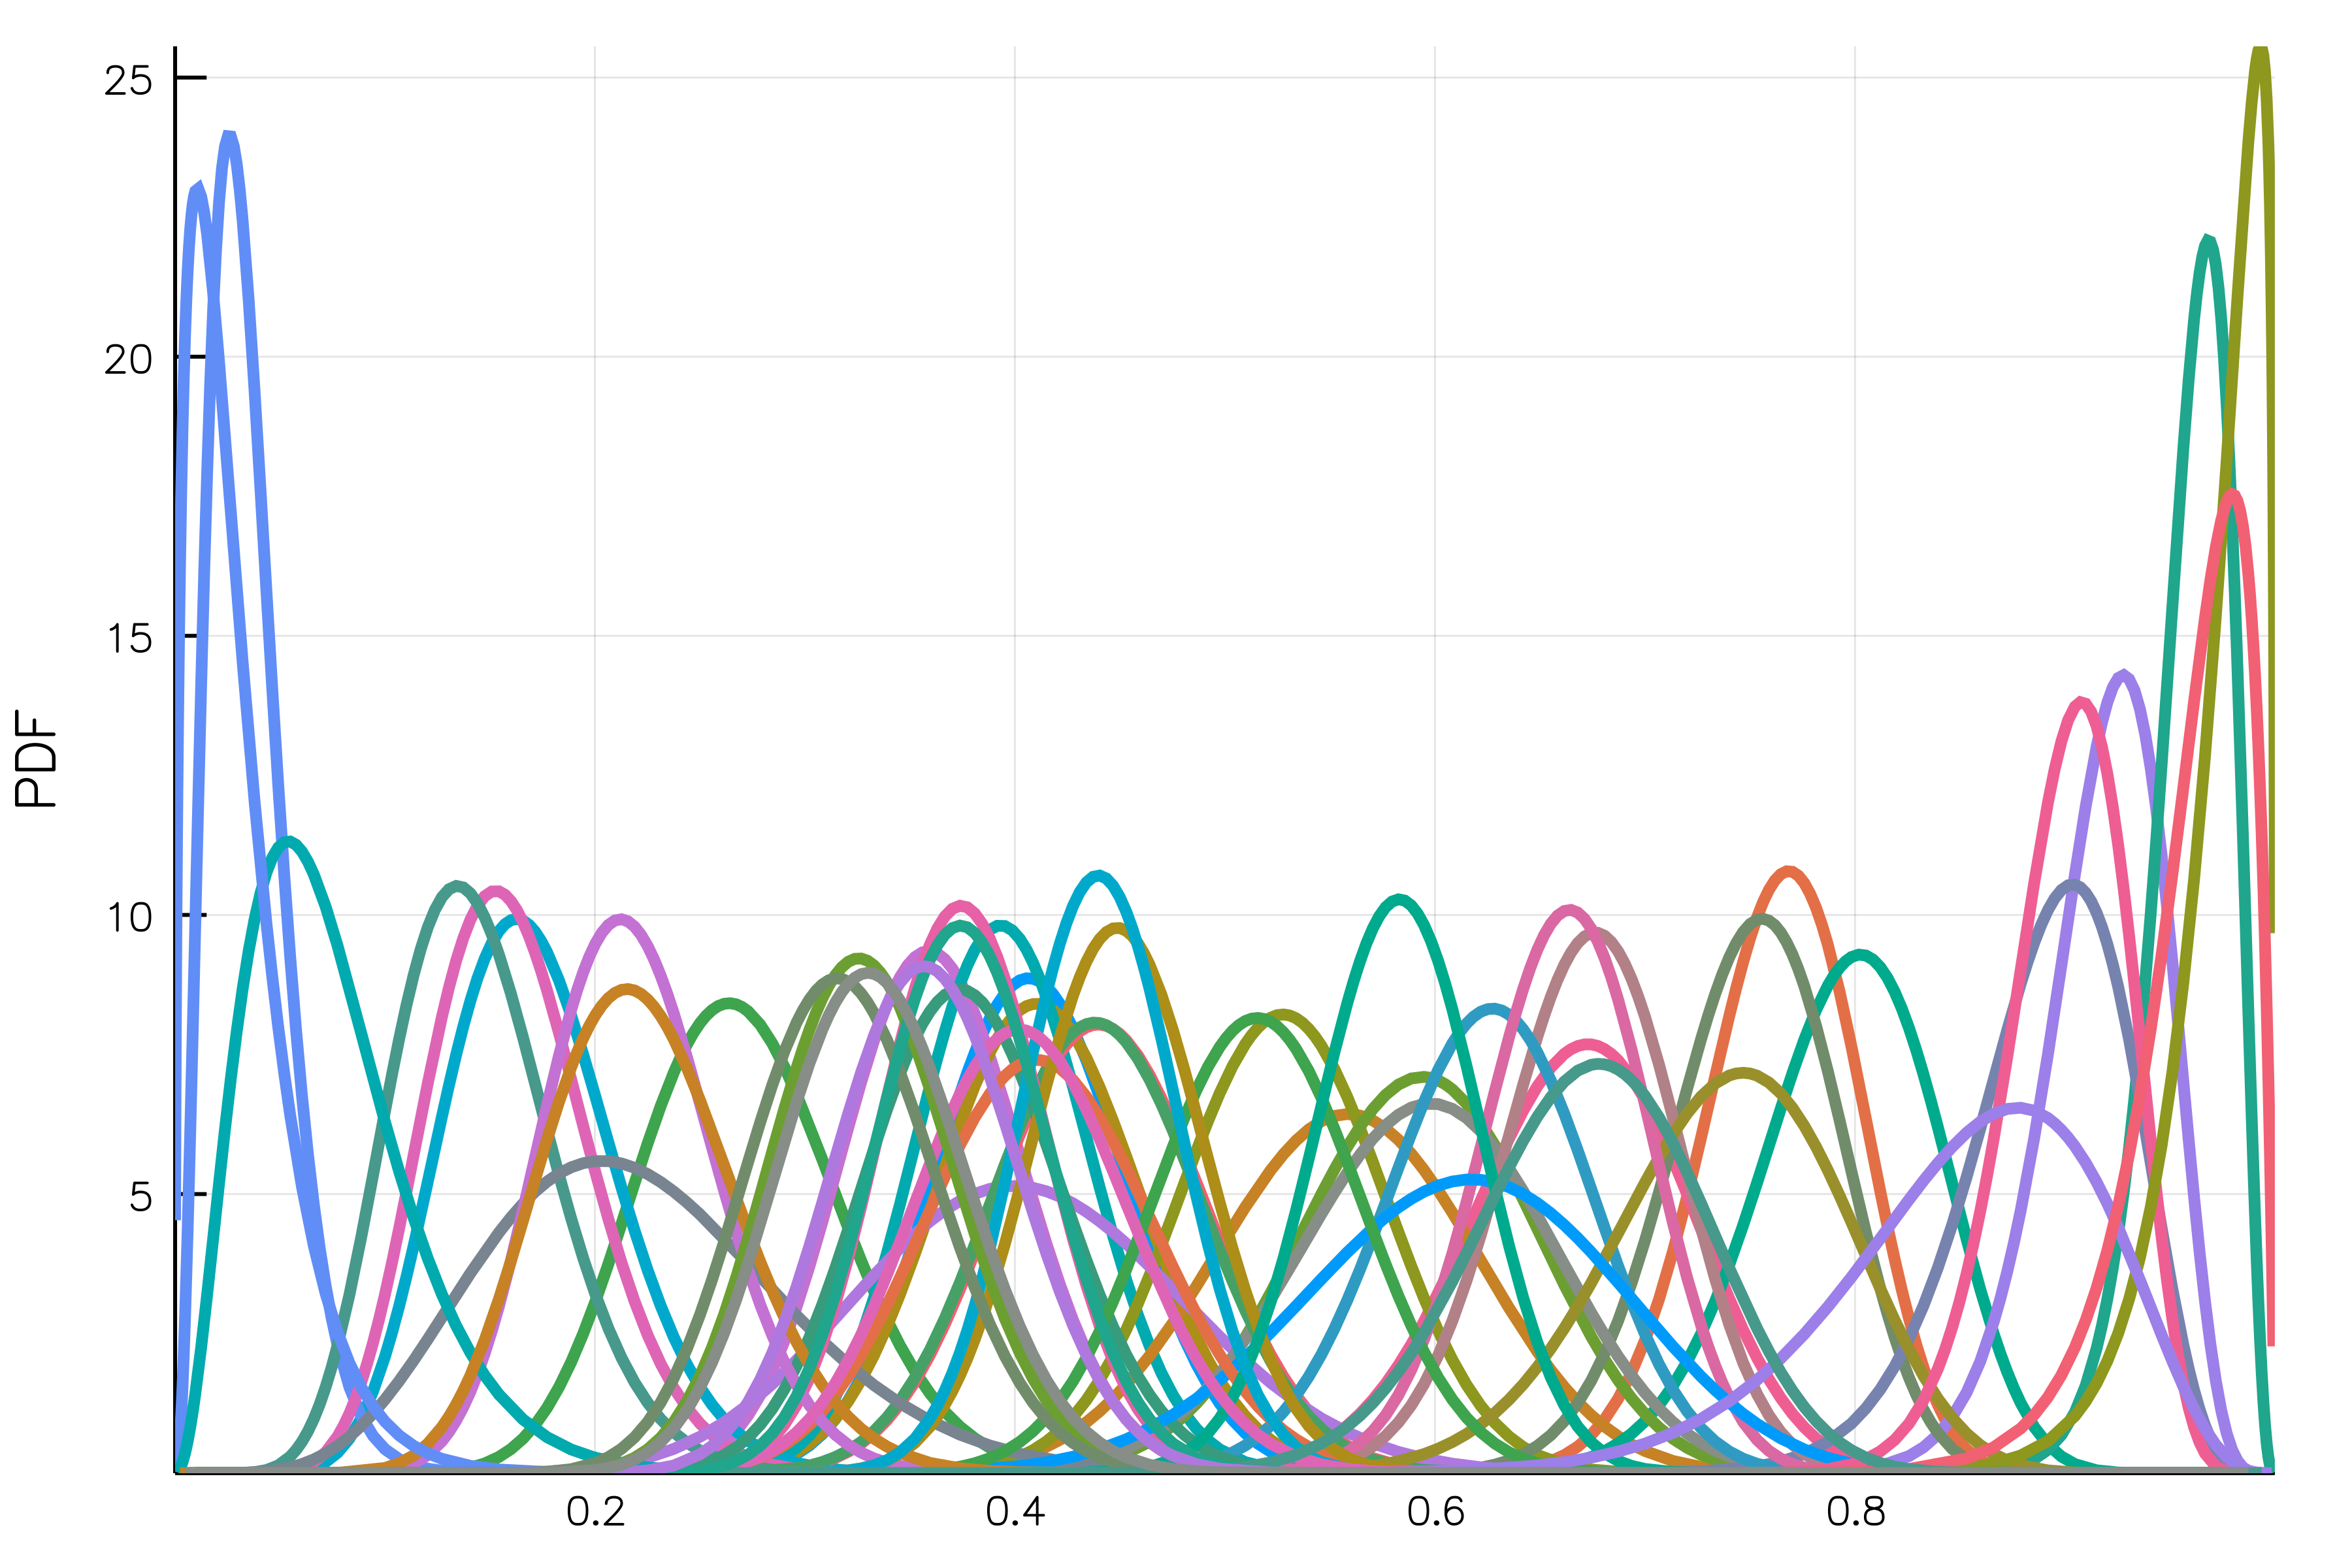
\includegraphics[width=\textwidth]{ims/beta100.png}
  \caption{Distribuições Beta para 50 agentes}
  \label{fig:betas100}
\end{figure}


A cada iteração da simulação um dos agentes vai ser escolhido e vai interagir
com um de seus vizinhos, a princípio num grafo completo imposto exogenamente
(estabeleço na condição inicial quais os vizinhos). A interação é assim em
díades, assíncrona (os agentes atualizam seus atributos em momentos distintos) e
sequencial (um agente atualiza por vez) \cite{wilensky2015introduction}. A
dependência dos resultados em relação ao número de agentes e de crenças vai ser
explorada. Estamos interessados nas alterações ao longo prazo (em termos de
iterações) da configuração dos \(x\) sob diferentes combinações de parâmetros,
tendo em vista as interações dos agentes \cite{acemoglu2011opinion}
\footnote{Como vamos definir longo prazo e analisar o modelo é tema da seção
  metodológica.}.

Quando os agentes interagem \(i\) atualiza sua opinião em alguma\footnote{Qual
  questão vão ``debater'' vai ser definido por meio de um sorteio sem viés. Uma
  outra implicação possível, a ser adicionada em trabalhos futuros, é considerar
  um viés nessa seleção, o que representaria saliência no sentido dado por
  \citeonline{zaller1992simple}: qual questão os agentes estão dando atenção,
  isto é, qual questão está mais acessível na memória deles.} questão segundo as
equações 2.3 e 2.4. Dado que os agentes agora tem um conjunto de opiniões é
plausível considerar que um conjunto de agentes tenham determinadas opiniões em
que eles tenham maior certeza, identificação, ou centralidade para o seu perfil
ideológico. Sendo assim na condição inicial alguma proporção de agentes tem uma
questão no seu perfil \(I\) cujos \(\sigma\) associados são aproximadamente zero. Com
isso buscamos analisar o papel de agentes ``inflexíveis'' na dinâmica
populacional. A proporção de agentes intransigentes ou inflexíveis é assim um
parâmetro da simulação.

Os agentes também vão reconsiderar suas opiniões e certezas sobre as questões
segundo uma probabilidade \(\rho\). Do ponto de vista teórico, estamos considerando
a possibilidade de fatores não relacionados à influência social levarem o agente
a mudar seu posicionamento sobre questões \cite{flache2017, lorenz2017modeling}.
Do ponto de vista metodológico, \citeonline{macy2015signal} argumenta que
pequenas perturbações no comportamento local dos agentes pode levar a mudanças
drásticas nas propriedades sistêmicas. Particularmente, consideram que adicionar
ruído pode: eliminar equilíbrios frágeis, o que reduz o conjunto de resultados e
tornando-os mais previsíveis; e embora aumente a heterogeneidade local isso pode
acabar facilitando interações sociais que reduzem a diversidade global
\cite[p.323]{macy2015signal}. A nova opinão é sorteada independentemente da
opinião anterior do agente. Contudo, no caso em que o agente seja intransigente
na questão ele não será sujeito ao efeito do ruído.


\section{Parâmetros-Chave}

Os parâmetros-chave para configuração e inicialização do modelo, cujos valores
seguem \citeonline{martins2008continuous}, \citeonline{deffuant2000mixing} e
\citeonline{lorenz2017modeling}, são:

\begin{itemize}
\item A população de \(500 < N < 5000\) agentes;
\item O número de questões \(1 \leq \text{n\_issues} \leq 10\); 

\item As incertezas \(0.01 \leq \sigma_i \leq 0.5\);
  \begin{itemize}
  \item Agentes intransigentes vão ter uma de suas opiniões com incerteza
    próxima a zero (\(1e-15\));
  \end{itemize}

\item O parâmetro de confiança \(0.1 \leq p \leq 0.99\);
  
\item A proporção de agentes intransigentes \(0.0 \leq (\text{p\_intran}) \leq 0.1\);

\item A probabilidade de reconsideração \(0.0 \leq \rho  \leq 0.1\);
  
\end{itemize}

\section{Inicialização e Iteração}

A inicialização da simulação depende dos parâmetros-chave apresentados. Na
condição inicial temos uma população de \(N\) agentes, que tem por atributos: um
conjunto de pares \(I_i = ((o_{i,1},\sigma_{i,1}^2), \ldots, (o_{i,n},\sigma_{i,n}^2))\), onde
o número de questões, \(n\), é uma variável global, cada \(o\) é retirado de uma
distribuição Beta(\(\alpha,\beta\)), onde cada agente tem um \(\alpha\) e um \(\beta\) próprio,
com valores\footnote{Paramêtros com valores \(\leq\) 1 ou geram distribuições de
  formato uniforme, quando \(\alpha = \beta = 1.0\), ou com formato de U. Quanto ao
  limiar superior, o valor de 100 permite que tenhamos agentes com distribuições
  centralizadas em ambos os extremos, dado que a média \(\mu\) é dada por
  \(\frac{\alpha}{\alpha + \beta}\), de forma que a média mínima é 0.011.} entre 1.1 e 30; o
\(\sigma^2\) é uma variável global ; um posicionamento ideológico, ou ponto ideal,
\(x_i = \frac{1}{n} \sum_{k = 1}^n o_{i,k} \); e um conjunto de vizinhos, o qual
depende de qual a rede os agentes estão. Uma determinada proporção de agentes,
contudo, vai ter um \(\sigma_i = (1e-15 ) \approx 0.0 \). Qual em particular é sorteado de
seu \(I\). Quantos agentes são intransigentes é dado por \(\text{p\_intran}\).

 Uma iteração da simulação, a
passagem de digamos \(t=2\) para \(t=3\), é dada pela aplicação de dois
procedimentos: a atualização via influência social e a atualização aleatória.
Uma repetição da simulação é a aplicação iterativa desses dois procedimentos ao
longo de um tempo \(t \).

O procedimento de influência social é o seguinte: escolhemos um agente \(i\) da
população. Então escolhemos um de seus vizinhos, \(j\). Sorteamos uma das
questões \(k \in (1,\ldots,n)\), e logo em seguida selecionamos os
\((o_{i,k},o_{j,k})\) e \((\sigma_{i,k}^2,\sigma_{j,k}^2)\) correspondentes à questão. A
partir daqui temos duas opções, \(i\) atualiza \(o_{i,k}\) segundo as equações
2.3 e 2.4. Essa regra é um parâmetro global da simulação, o que significa que a
cada repetição todos os agentes atualizam suas crenças segundo a mesma regra.

Ademais, temos o ruído. Novamente escolhemos um agente \(i\) da população.
Sorteamos uma questão e selecionamos \(o\) e \(\sigma^2\) correspondentes. Se o
agente é intransigente naquela questão então ele não muda de opinião. Sorteamos
um \(\xi\) retirado de uma distribuição uniforme \(U([0,1])\) e se \(\xi < \rho\) \(i\)
muda \(o\) para um valor retirado de outra distribuição uniforme (U[0,1]). Os
\(x_i\), o objeto de interesse de análise, são atualizados sempre que ocorrerem
mudanças nas crenças dos agentes.

\section{Metodologia de Análise}

Dentre as diversas formas de analisar um ABM a análise de sensibilidade global
se destaca como uma forma de ter uma compreensão ampla, geral, do comportamento
do modelo \cite{north2007managing}. O primeiro passo da análise envolve, então,
 ter uma compreensão geral do comportamento do modelo para então passarmos
para regiões particulares do espaço de parâmetros.

Contudo, o alto custo computacional de varrer esse espaço de parâmetros faz com
que só seja possível realizarmos uma análise global, na maioria dos casos, se
seguirmos métodos formais da literatura de análise de sensibilidade
\cite{railsback2012agent}. Esses métodos trazem o benefício de determinar como
selecionar subconjuntos de todas as combinações de parâmetros, reduzindo o
número de realizações necessárias da simulação e de trazerem formas sistemáticas
de interpretar os resultados \cite{railsback2012agent}.

Quanto à amostragem uma estratégia comum são as parametrizações de Monte Carlo:
sortear valores de parâmetros usados para as realizações das simulações a partir
de distribuições uniformes nos intervalos de valores dos parâmetros
\cite{laver2011party}. O problema dessa estratégia é que o espaço de parâmetros
não é coberto igualmente, havendo a possibilidade de pontos de acumulação ou
espaços vazios \cite{pereda2017brief}.

\citeonline{saltelli2008global} argumenta que para manter uma dispersão equitativa
dos pontos no espaço de parâmetros é necessário um algoritmo que enviese a
seleção de novos pontos para mantê-los afastados dos pontos já presentes. Desta
forma vamos usar o método de Saltelli de amostragem, dado que garante a partição
equitativa do espaço de parâmetros \cite{herman2017salib}. Especificamos então
um \(n\) base a partir do qual o ``sampler'' gera n * (2d + 2), onde \(d\) é o
número de parâmetros. No nosso caso \(d = 6\), pois vamos ter como parâmetros :
N (população), número de questões (codificado como n\_issues ), \(p\), \(\sigma\), a
proporção de agentes intransigentes (codificado como p\_intran)
\(\rho\). Para garantir um coeficiente de erro baixo no cálculo
subsequente dos índices de sensibilidade especificamos um \(n\) base de
\(5000\), de forma que para cada caso rodamos \(70.000\) parametrizações.


\begin{figure}[h]
    \centering
    \begin{subfigure}[b]{0.49\textwidth}
      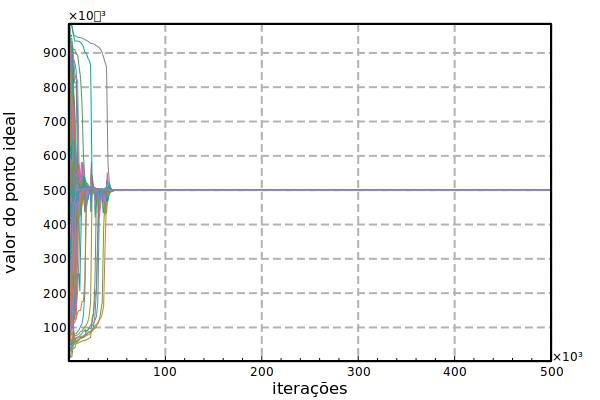
\includegraphics[width=\textwidth]{ims/timeseries1.png}
      \caption{\( \sigma = 0.1\) }
    \end{subfigure}
    \begin{subfigure}[b]{0.49\textwidth}
      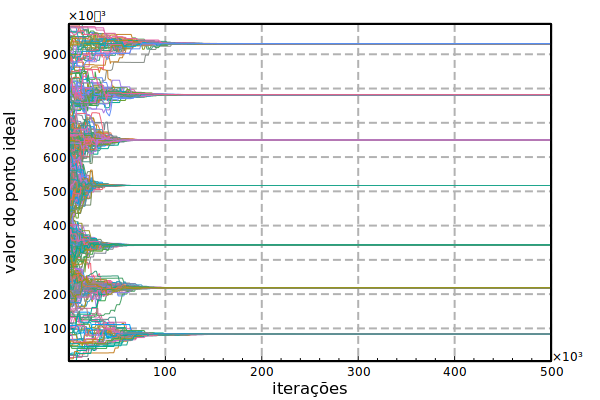
\includegraphics[width=\textwidth]{ims/timeseries2.png}
       \caption{\(\sigma = 0.02\) }
      \end{subfigure}
      \caption{Evolução dos pontos ideais dos agentes ao longo de duas realizações.
        Parametrização: \(  N = 500, p = 0.9, \rho = 0.0, n\_issues = 1 , p\_intra
        n= 0.0 \)}
      \label{fig:tseries1}
    \end{figure}
    
Uma vez especificado o método de amostragem especificamos uma medida do sistema
para que possamos analisá-lo \cite{railsback2012agent}. Escolhemos o desvio
padrão dos pontos ideais após \(1.000.000\) iterações como output para
análise\footnote{Testamos diversas parametrizações com n\_issues \(= 1\) e
  observamos que a partir de \(50.000\) iterações a implementação replica os
  resultados de \citeonline{martins2009bayesian}.}, dado que nos diz o quão
concentradas ou dispersos são os pontos ideais da população. Uma outra opção de
medida do sistema seria o número de opiniões finais após as iterações. Contudo,
teríamos que estabelecer um \(N\) base, pois de outra forma esse parâmetro
explica quase que totalmente o valor do output a ser analisado. No primeiro
gráfico da figura \ref{fig:tseries1} temos um desvio padrão próximo zero, e um
único posicionamento ideológico final. Já no segundo gráfico precisáriamos
arredondar os pontos ideais finais, entre 1 e 6 casas decimais, para
chegarmos a conclusão que existem cerca de 6 pontos de convergência. Se não arrendondarmos o
resultado final teriamos uma medida próxima de 500 pontos ideais. O desvio
padrão, contudo, nos indica a dispersao dos pontos ideais, pois tem valor de
aproximadamente 0.24, próximo ao da condição inicial. A figura \ref{fig:tseries1}
deixa claro, portanto, que as medidas são complementares, mas como estamos
interessados no papel do \(N\) vamos começar com a análise com o desvio padrão
dos pontos ideais como medida do sistema.


Para a análise, seguimos \citeonline{ten2016sensitivity} e combinamos
histogramas da medida do sistema, gráficos de dispersão e índices de
sensibilidade.Os índices de sensibilidade utilizados são os índices de
Sobol\footnote{Tanto a amostragem quanto a análise de sensibilidade são feitas
  usando o pacote de Python SALib \cite{herman2017salib}.}, particularmente
índices de Sobol de primeira ordem e totais \cite{saltelli2008global}. Os
índices de Sobol decompõe o impacto dos parâmetros na variância do
\textit{output} de interesse. Os índices de primeira ordem incluem contribuições
lineares e não-lineares dos parâmetros, mas não efeitos interativos
\cite{ten2016sensitivity}. Já índices totais incluem todos os efeitos de ordem
maior decorrentes das interações entre os parâmetros \cite{saltelli2008global}.

\section{Resultados}

\todo[inline,color = yellow!10]{A partir daqui vai ser reescrito por causa das
  modificações no modelo.}

Rodamos então \(70.000\) parametrizações por \(1.000.000\) de iterações tendo
por \(Y\), o \textit{output} de interesse, o desvio padrão  dos pontos ideais da
população (\(\text{Ystd}\)) após as iterações. São \(6\) os parâmetros de input
: o número de agentes (\(N\)), o número de questões (\(\text{n\_issues}\)), o
parâmetro de confiança (\(p\)), a incerteza (\(\sigma\)),  o ruído \(\rho\), e a
proporção de agentes intransigentes (\(p\_intran\)) nos
limiares apresentados na seção Parâmetros-Chave.

Como uma primeira aproximação do comportamento geral do modelo, a Figura
\ref{fig:hists1} apresenta a dispersão dos pontos ideais na condição inicial e
ao fim das simulações para cada parametrização.

\begin{figure}[h]
    \centering
    \begin{subfigure}[b]{0.49\textwidth}
      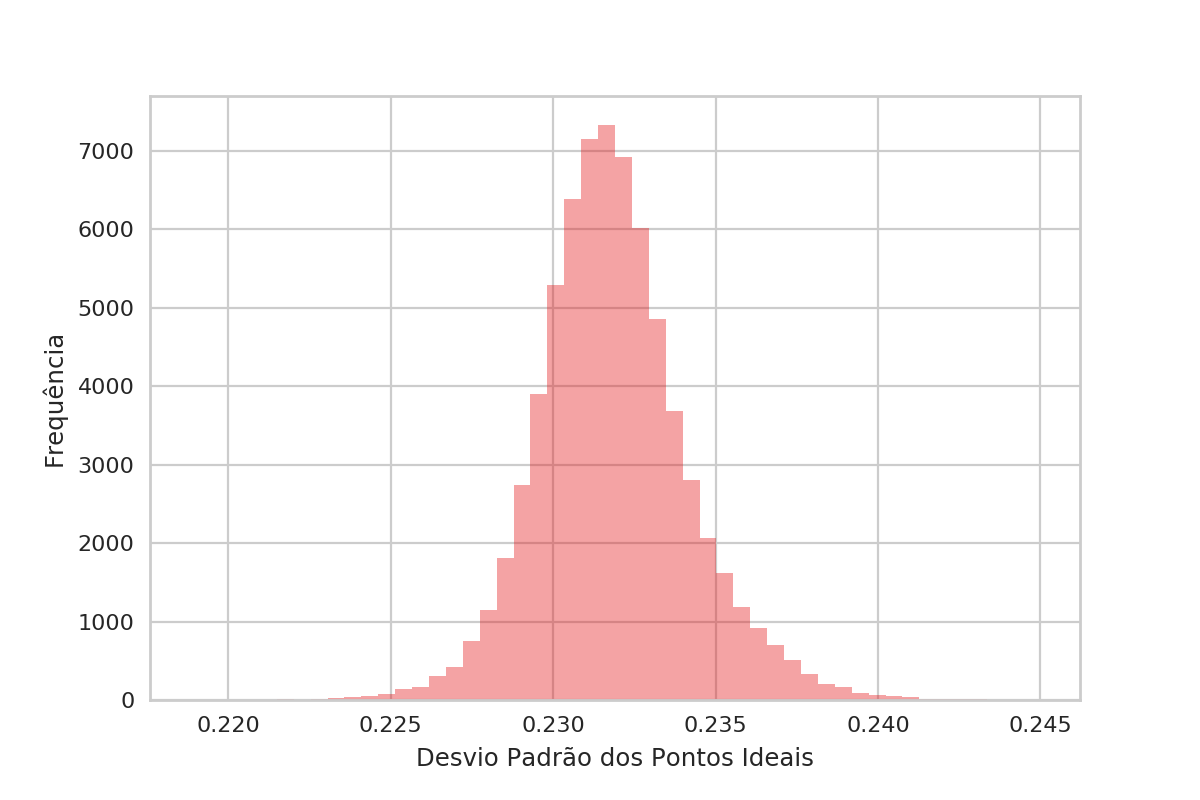
\includegraphics[width=\textwidth]{ims/diststdinit.png}
      \caption{Condição inicial}
    \end{subfigure}
    \begin{subfigure}[b]{0.49\textwidth}
      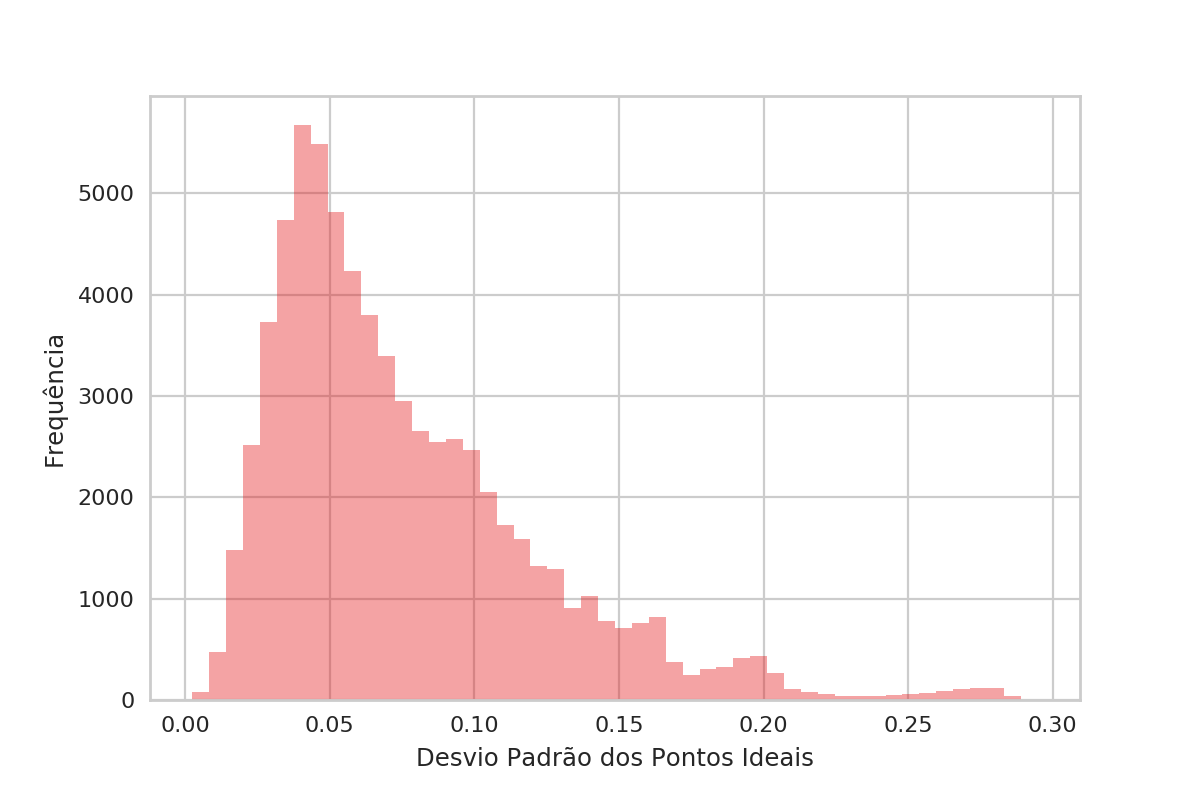
\includegraphics[width=\textwidth]{ims/distY.png}
       \caption{Após 1.000.000 iterações}
      \end{subfigure}
      \caption{Desvio padrão dos pontos ideais das populações para cada parametrização}
      \label{fig:hists1}
    \end{figure}
    

%
%
%\begin{figure}[H]
%  \centering
%  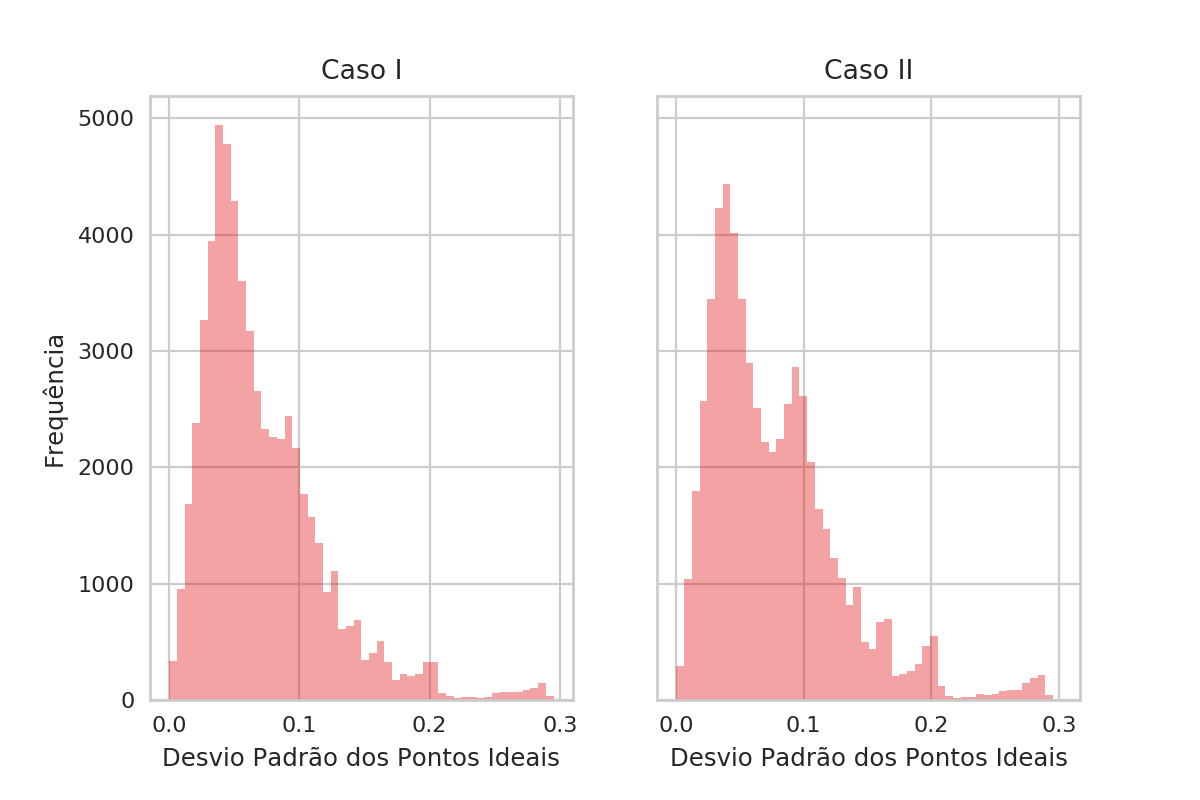
\includegraphics{ims/distYs.png}
%  \caption{Output (desvio padrão dos pontos ideais) }
%  \label{fig:Yshist}
%\end{figure}

    A Figura \ref{fig:hists1} nos leva a interpretar que a aplicação iterativa
    do procedimento do modelo, deixa a distribuição de opiniões menos dispersa,
    com uma maior concentração das parametrizações em outputs de baixa dispersão
    (entre 0.0 e 0.1). Isso condiz com as regras de atualização (assimilativa,
    mas na qual agentes distantes tem pouco impacto na opinião um dos outros) e
    com o fato dos agentes terem por vizinhos todos os outros agentes. Isto é,
    os agentes ao interagirem ou ficam mais parecidos ou não são influenciados.
    O modelo tem assim uma forte tendência assimilativa, ao menos num grafo completo.
    Contudo, a figura não nos informa qual parâmetro é responsável por isso, ou
    quais os valores de concentração (centrais ou extremos).

    A primeira pergunta pode começar a ser respondida por meio de gráficos de
    dispersão. A partir da Figura \ref{fig:scatter1} podemos inferir que há uma
    relação negativa entre os parâmetros \(\text{n\_issues}, p, \sigma \) e a
    dispersão dos pontos ideais (\( \text{Ystd}) \). A relação entre \(p\) e
    \(\sigma\) são explicadas pelo fato de agentes que ``confiam'' mais na opinião
    dos outros agentes e são mais incertos vão convergir mais rápido para a
    mesma opinião.

\begin{figure}[H]
    \centering
    \begin{subfigure}[b]{0.49\textwidth}
        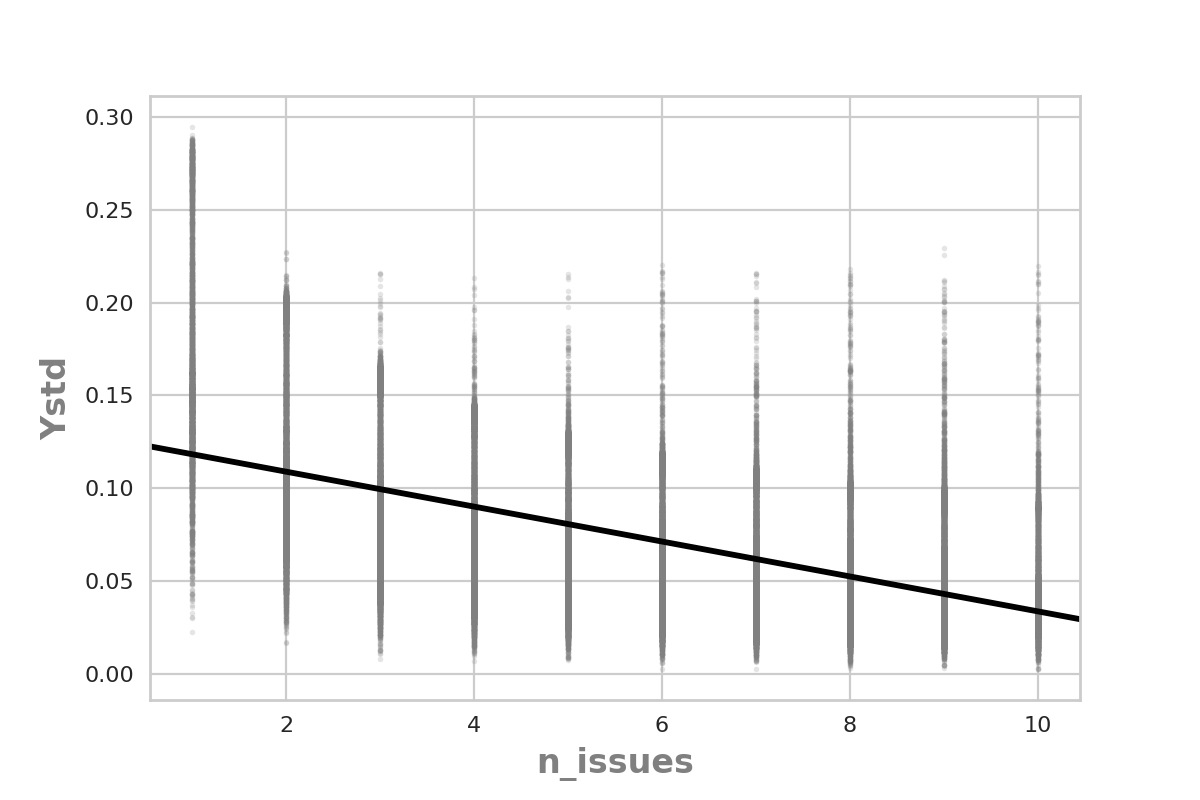
\includegraphics[width=\textwidth]{ims/mutoregressions/regressionmutatingon_issues.png}
    \end{subfigure}
    \begin{subfigure}[b]{0.49\textwidth}
        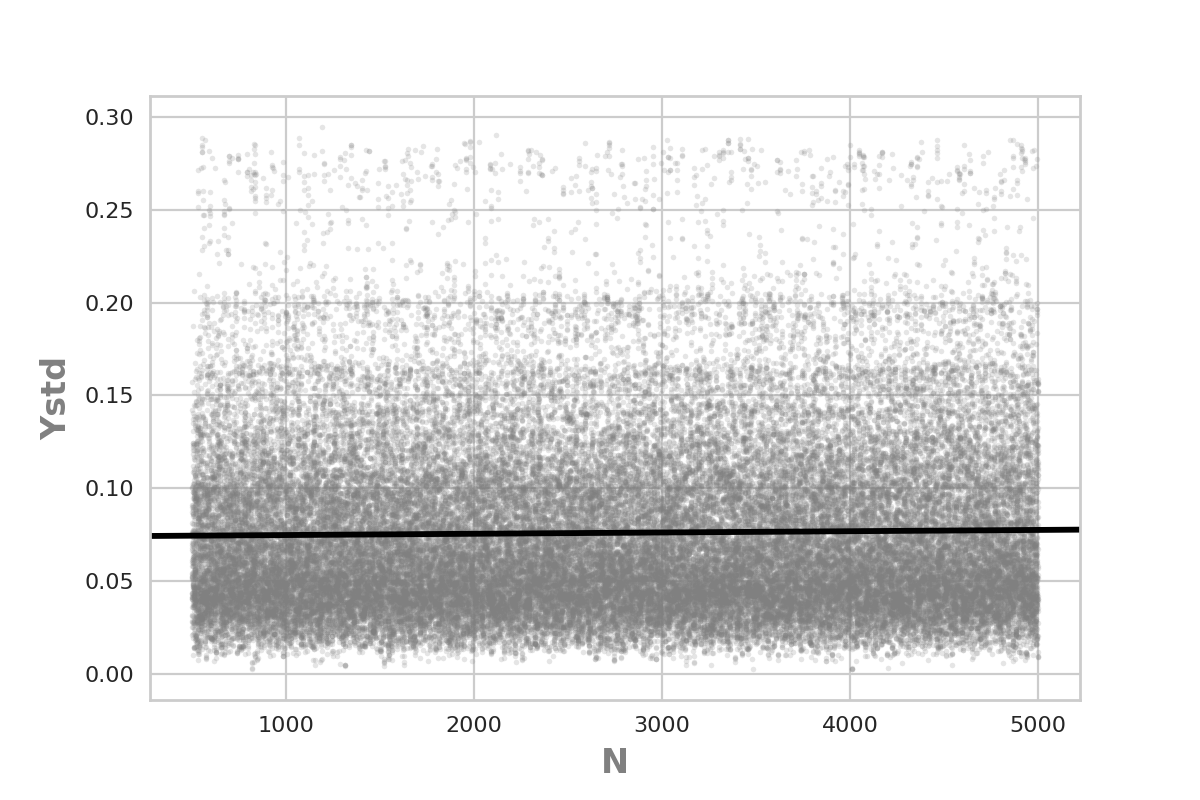
\includegraphics[width=\textwidth]{ims/mutoregressions/regressionmutatingoN.png}
    \end{subfigure}

    \begin{subfigure}[b]{0.49\textwidth}
        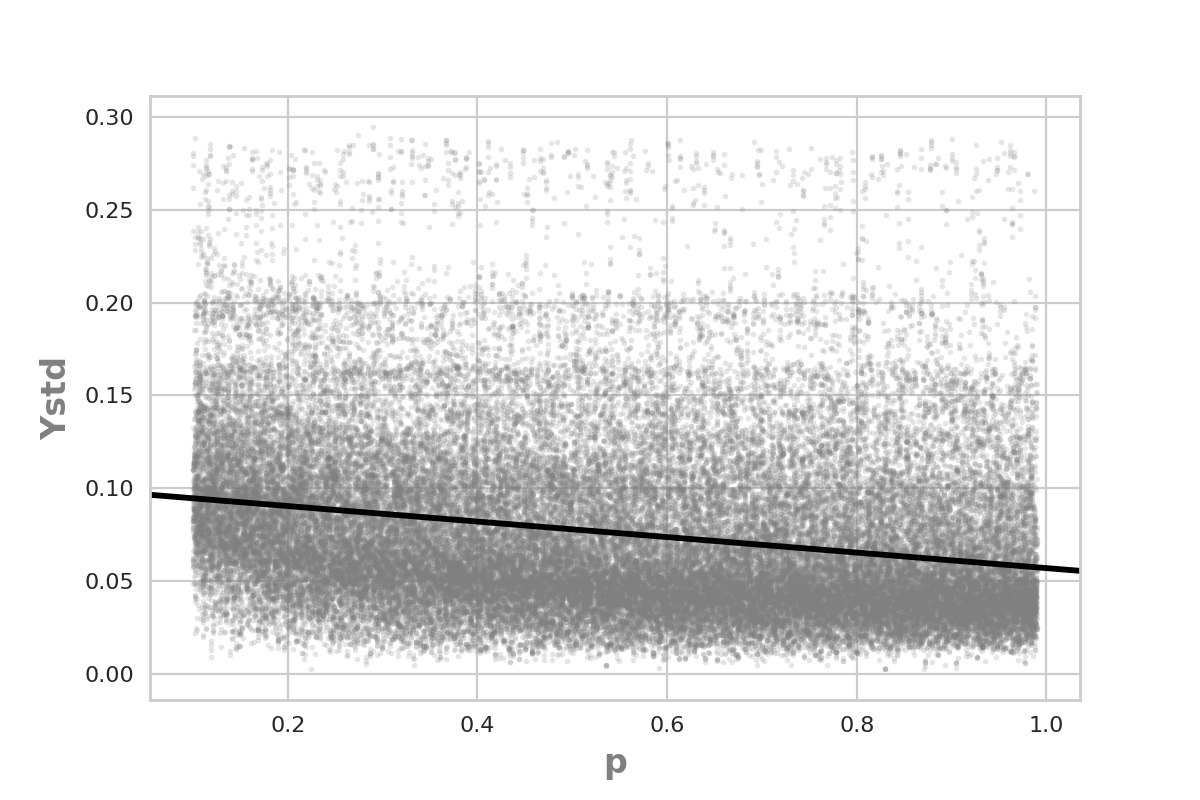
\includegraphics[width=\textwidth]{ims/mutoregressions/regressionmutatingop.png}
      \end{subfigure}
          \begin{subfigure}[b]{0.49\textwidth}
            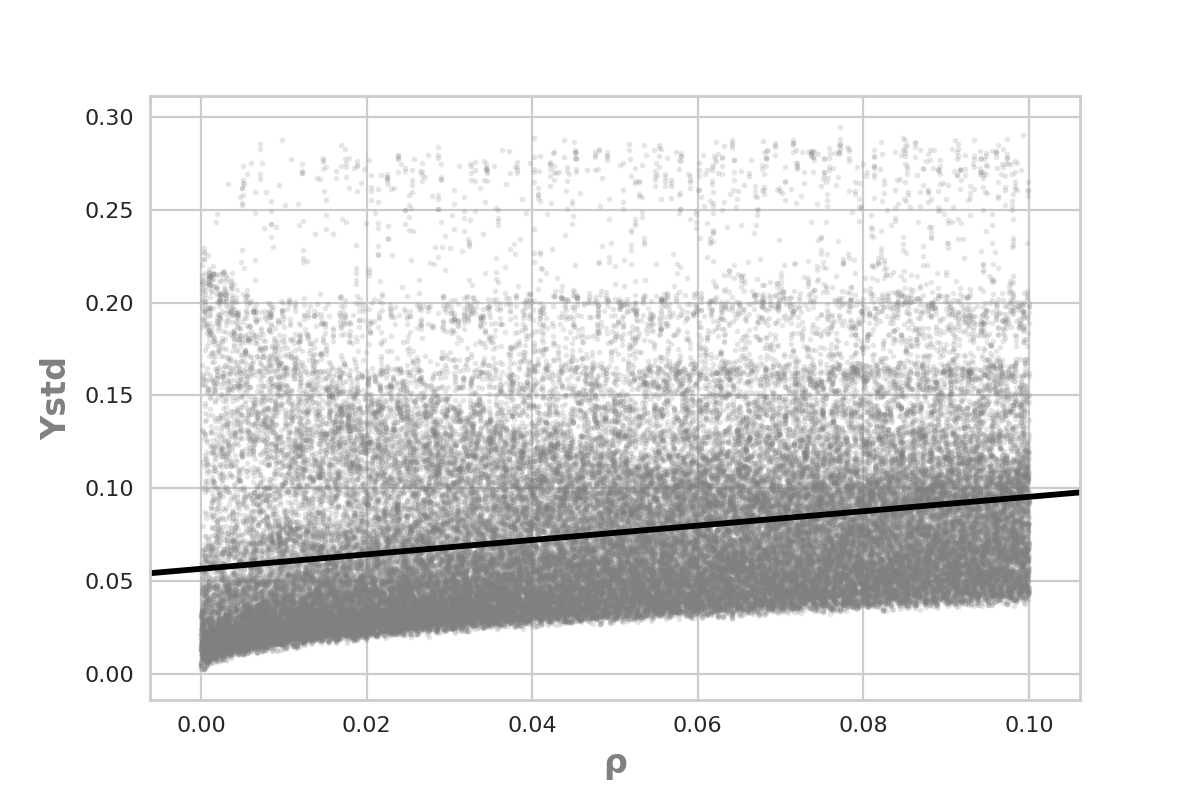
\includegraphics[width=\textwidth]{ims/mutoregressions/regressionmutatingorho.png}
      \end{subfigure}

                \begin{subfigure}[b]{0.49\textwidth}
            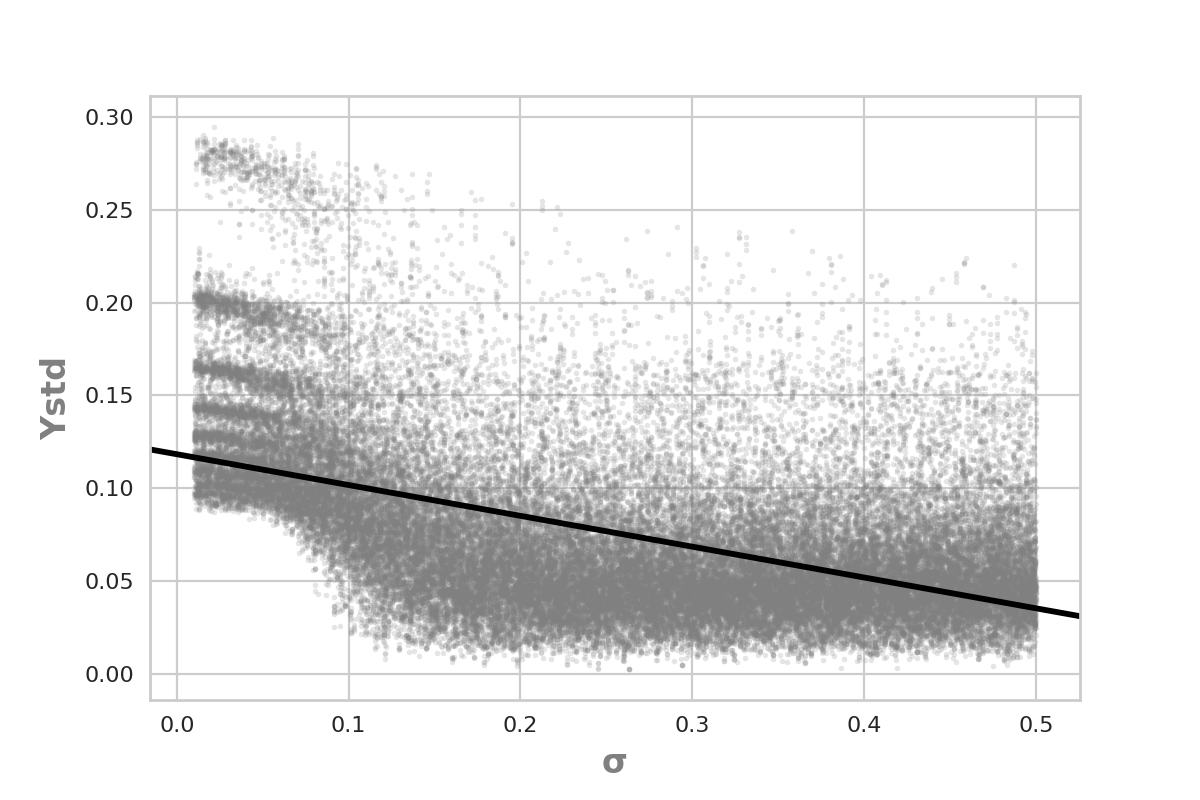
\includegraphics[width=\textwidth]{ims/mutoregressions/regressionmutatingosigma.png}
          \end{subfigure}
                \begin{subfigure}[b]{0.49\textwidth}
            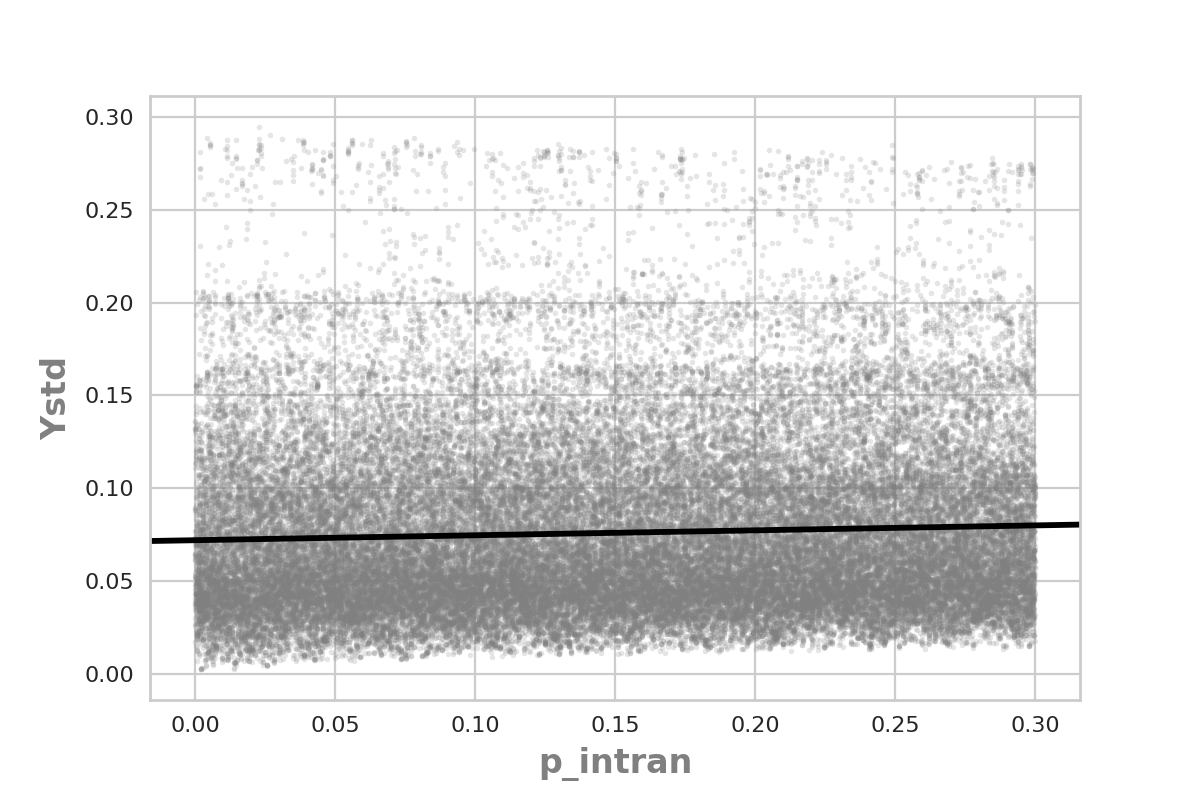
\includegraphics[width=\textwidth]{ims/mutoregressions/regressionmutatingop_intran.png}
    \end{subfigure}
    \caption{Gráfico de dispersão para 70.000 parametrizações no Caso I.}
    \label{fig:scatter1}
    Fonte:Elaboração própria.
\end{figure}

\todo[inline,color = yellow!10]{Tou devendo de explicar a relação negativa entre
numero de questões e dispersão.}

O parâmetro \(\rho\), o ruído, por sua vez, tem uma relação positiva com a
dispersão do sistema. Interessante notar, contudo, que o tamanho da população
parece não ter relação com o desvio padrão dos pontos ideais da população.

A intensidade dos parâmetros na variância da medida do sistema (Ystd) fica mais
claro na Figura \ref{fig:sobol1}:

\begin{figure}[H]
  \centering
  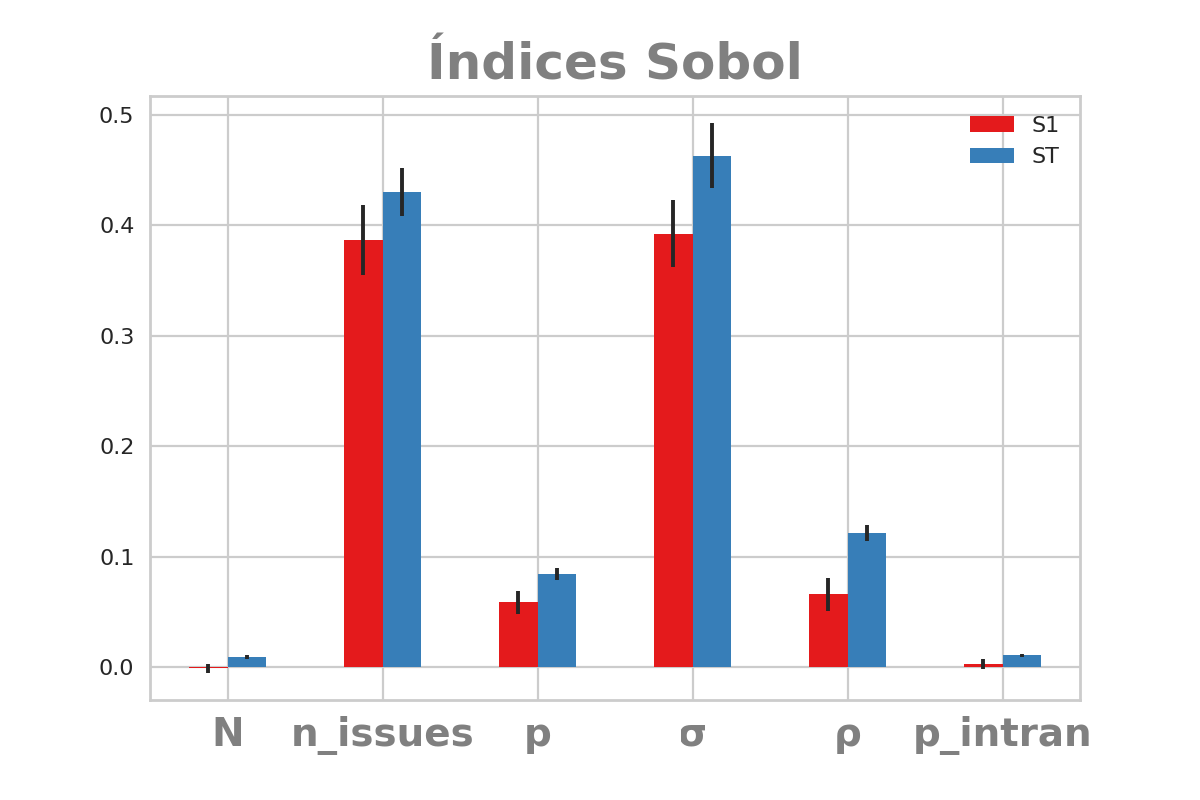
\includegraphics{ims/barplotmuto5k.png}
  \caption{Índices de Sobol de sensibilidade}
  \label{fig:sobol1}
\end{figure}

Como mostra a Figura \ref{fig:sobol1} o parâmetro \(N\) não tem impacto sobre a
variância de \(Ystd\), de forma que podemos tratá-lo como uma constante para
análise subsequentes. A figura mostra que a maior parte da variância na
dispersão dos pontos ideais pode ser explicada pelos parâmetros \(\sigma\) e
\(\text{n\_issues}\). Além disso há pouca diferença entre os índices de primeira
ordem e os índices totais, o que implica que há poucos efeitos interativos entre
os parâmetros. Ademais, os coeficientes de erro são pequenos
\todo[color=yellow!10]{gerar tabela} tendo em vista que a análise foi feita a
partir de 70.000 parametrizações selecionadas por meio do método de Saltelli.

Um resultado contra-intuitivo, contudo, é o baixo valor de impacto do parâmetro
\(p\_intran\). A comparação entre as figuras \ref{fig:tseries1} e
\ref{fig:tseries2} sugere que esse resultado seja um artefato da medida Ystd.
Enquanto que na figura \ref{fig:tseries1} (a) o sistema converge para um único
valor, na figura \ref{fig:tseries2} a população oscila no espaço onde há mais
intransigentes. O parâmetro tem assim um impacto sobre a dinâmica.

\begin{figure}[h]
    \centering
    \begin{subfigure}[b]{0.49\textwidth}
      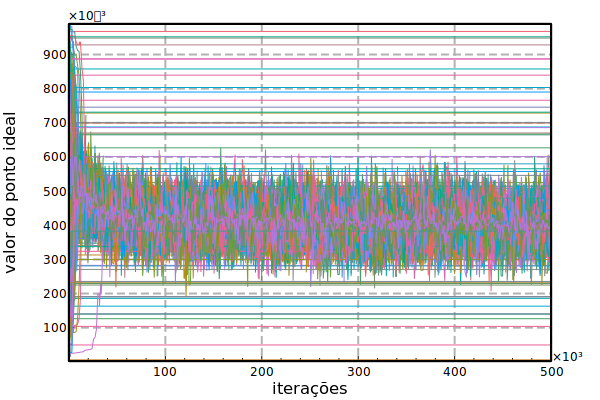
\includegraphics[width=\textwidth]{ims/timeseries3.png}
      \caption{\( \sigma = 0.1\) }
    \end{subfigure}
    \begin{subfigure}[b]{0.49\textwidth}
      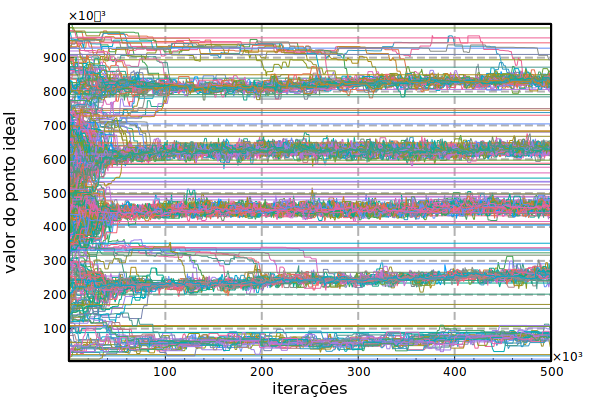
\includegraphics[width=\textwidth]{ims/timeseries4.png}
       \caption{\(\sigma = 0.02\) }
      \end{subfigure}
      \caption{Evolução dos pontos ideais dos agentes ao longo de duas realizações.
        Parametrização: \(p\_intran = 0.15 N = 500, p = 0.9, \rho = 0.0, n\_issues = 1 \)}
      \label{fig:tseries2}
    \end{figure}
    



%%% Local  Variables:
%%% mode: latex
%%% TeX-master: "master"
%%% End:
